We test the scalability with respect to data dimensionality and number of microclusters, using data generated by a \textit{Random Radial Basis Function} generator.

The scalability tests are performed in two different scenarios: one being an analysis of how it scales for different number of attributes (dimensions of the data points) using only 20 micro-clusters and the other one using 200 micro-clusters. The reason behind this is that the number of attributes and the number of final clusters for a specific purpose are two key factors which determine the complexity of \textit{Spark-CluStream}. The speed of the stream is controlled for 10000 points for every batch of data because it is easier to test the scalability when many computations have to be done.

Any application using Spark streaming assigns one core exclusively to handle the stream, therefore the minimum number of processors required is two, this also means that using 2 processors is equivalent to using a single processor to execute the application. The number of processors mentioned in these tests is the total, but the real number of processors used for the computations is that number minus one.


\begin{figure*}[!ht]
        \begin{minipage}[l]{1.0\columnwidth}
            \centering
             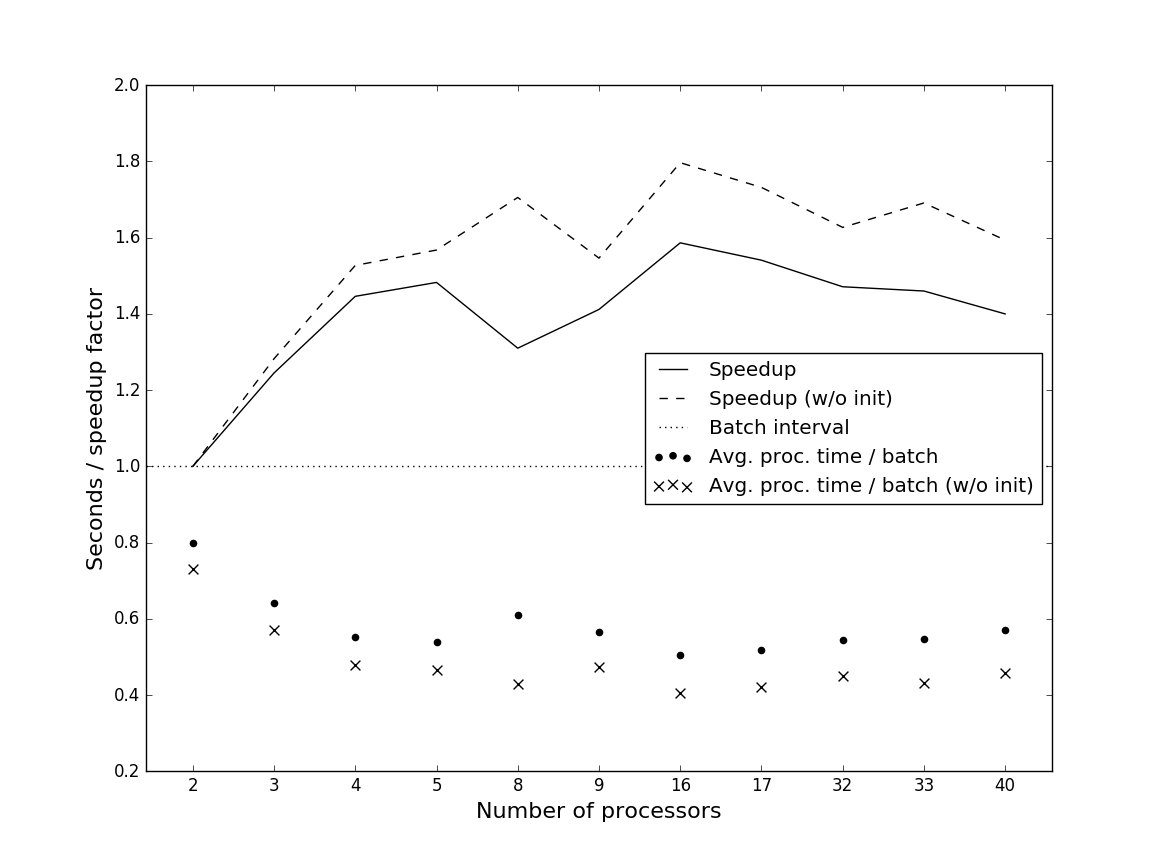
\includegraphics[width=0.9\columnwidth]{./styles/perf20-2.png}
            \caption{Dimension: $d$ = 2}
            \label{fig:perf20-2}
        \end{minipage}
        \hfill{}
        \begin{minipage}[r]{1.0\columnwidth}
            \centering
            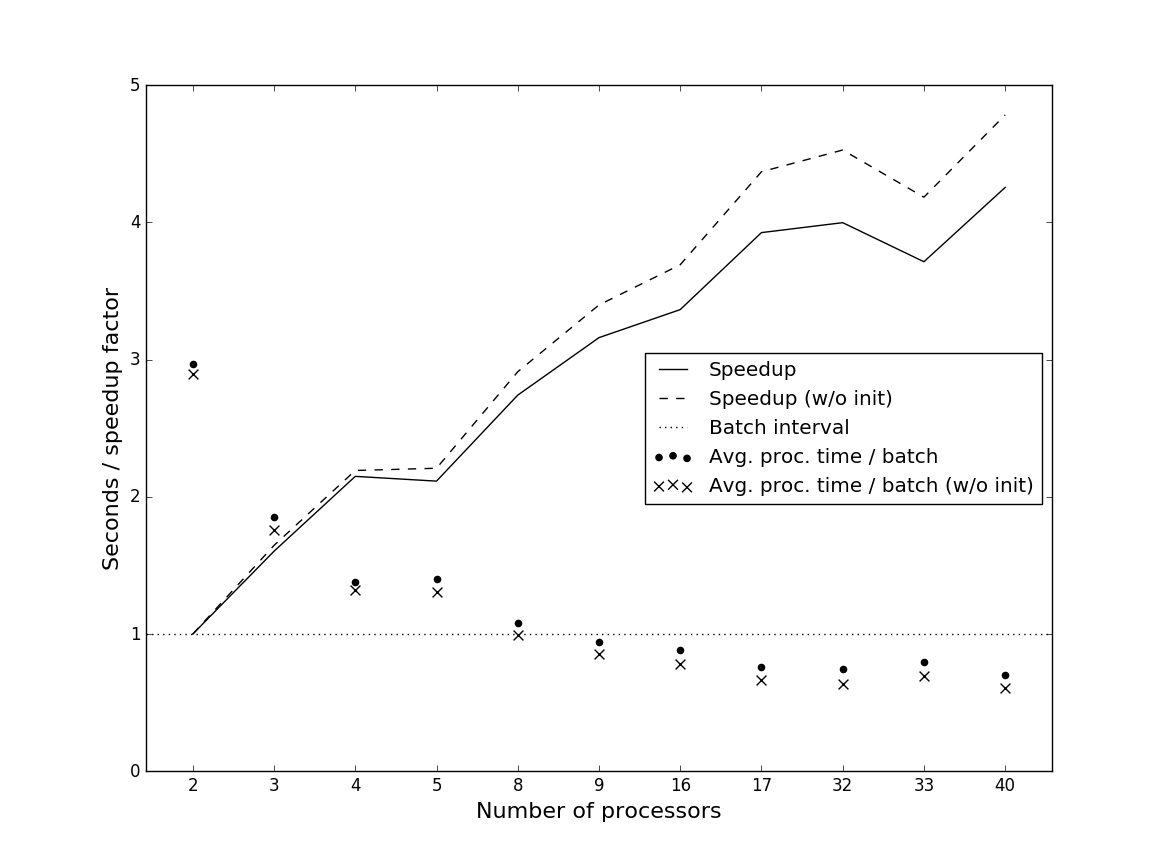
\includegraphics[width=0.9\columnwidth]{./styles/perf20-100.png}
            \caption{Dimension: $d$ = 100}\label{fig:perf20-100}
        \end{minipage}
        \captionsetup{labelformat=empty}
	\caption{Scalability-dimensionality comparison for Stream speed = 10000 and q = 20}
	 \label{fig:DS1quality}
\end{figure*}
\addtocounter{figure}{-1}
The charts here presented show the speedup obtained by increasing the number of processors from 2 to 40, which in reality means that 1 to 39 processors where used for the computations. It also shows the average processing time for each batch of data. Because the initialization takes the most amount of time, it is also convenient to show these values without considering that process: by doing so it is possible to see what would be the expected results for a longer run, where the initialization is no longer dominant. Finally it shows the interval time for which Spark process a new batch of data, in particular all these tests processed batch every second.


Figure \ref{fig:perf20-2} shows that using only 20 micro-clusters and 2 dimensions has poor scalability, not even being able to perform twice as fast as for a single processor (2 in total). Even for this high speed streaming, one processor is enough to process the batches of data before a new batch is processed, meaning that the setup is stable.

\begin{figure*}[!ht]
        \begin{minipage}[l]{1.0\columnwidth}
            \centering
             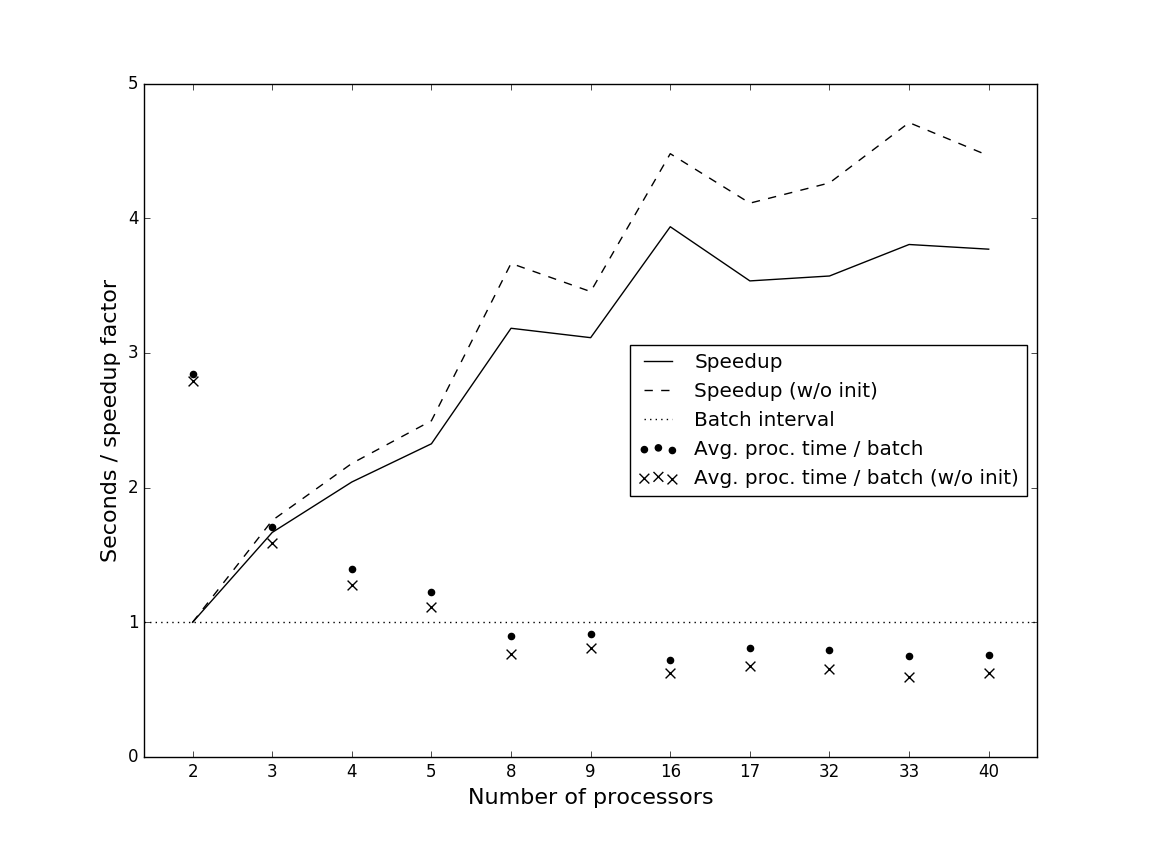
\includegraphics[width=0.9\columnwidth]{./styles/perf200-2.png}
            \caption{Dimension: $d$ = 2}
            \label{fig:perf200-2}
        \end{minipage}
        \hfill{}
        \begin{minipage}[r]{1.0\columnwidth}
            \centering
            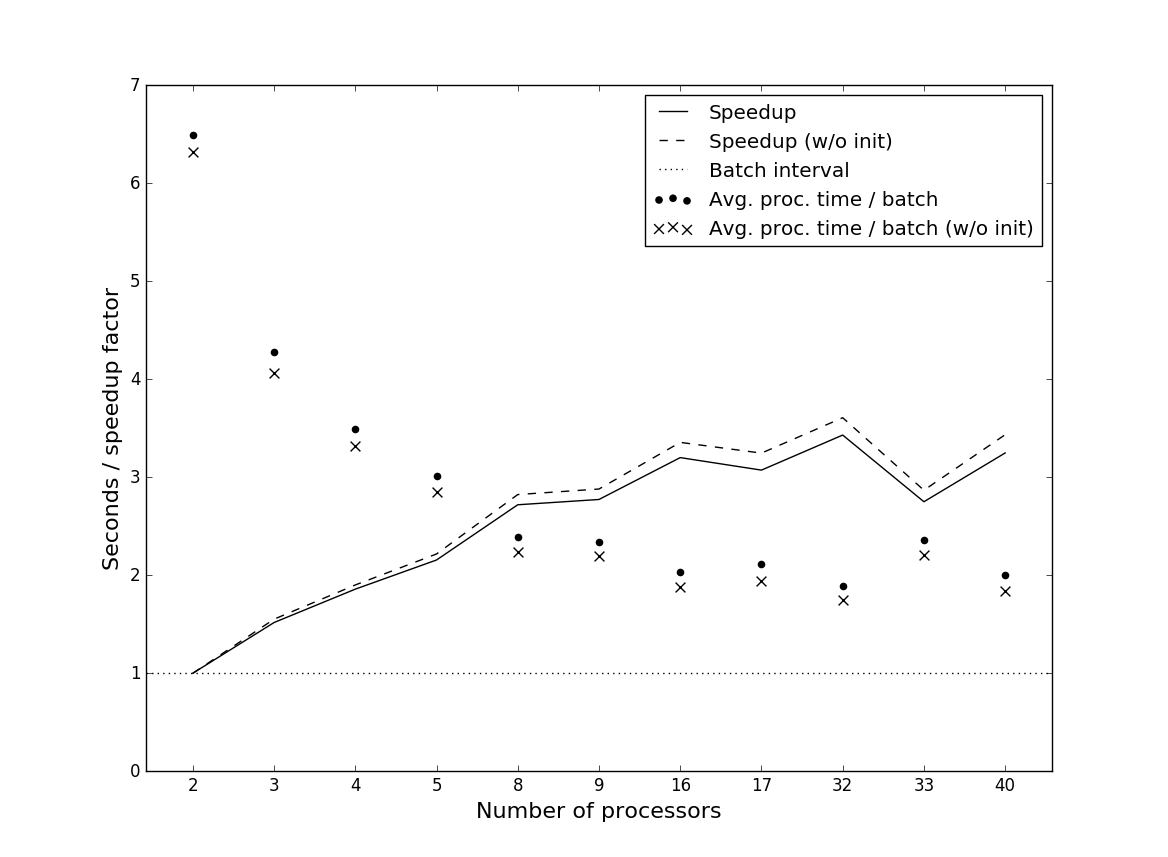
\includegraphics[width=0.9\columnwidth]{./styles/perf200-100.png}
            \caption{Dimension: $d$ = 100}\label{fig:perf200-100}
        \end{minipage}
        \captionsetup{labelformat=empty}     
        \caption{Scalability-dimensionality comparison for Stream speed = 10000 and q = 200}
        \label{fig:DS2quality}
\end{figure*}

\addtocounter{figure}{-1}
Increasing the dimensionality of the points increases the computational effort needed to process the points in every batch of data and here is where \textit{Spark-CluStream} shows its scalability, which is almost linear\footnote{By linear scalability does not mean it scales with a 1 to 1 ratio, but rather linearly proportional.} for up to 16-17 processors, as it can be seen in Figure \ref{fig:perf20-100}.  From the average processing time per batch, it can be seen that from 32 to 40 processors it does not improve much anymore and the speedup does not increase quasi-linearly anymore. Here a total of 9 processors were required to stabilize \textit{Spark-CluStream}. 


Interestingly, increasing the number of micro-clusters by a factor of 10 for 2 attributes resulted in good scalability, similarly to the scenario with 20 micro-clusters and 100 attributes. Here a total of 8 processors were enough for a stable run, as shown in Figure \ref{fig:perf200-2}.



Finally, when the number of clusters and the number of attributes are both increased significantly, Figure \ref{fig:perf200-100} shows for \textit{Spark-CluStream} quasi-linear scalability but this time only up to about 8-9 processors. After that point, the speedup slows down showing almost no improvement after 16 processors. This test never reached a stable configuration.


\subsection{Performance}

In this section, the scalability of \textit{Spark-CluStream} is compared to that of \textit{StreamDM-CluStream} and Spark's \textit{Streaming K-Means} unsing the Spark cluster setup for $q=20$ and $d=2,100$, for the $CluStream$ method. Also, a test on a signle machine is performed.


\begin{figure}[h!]
 \centering
 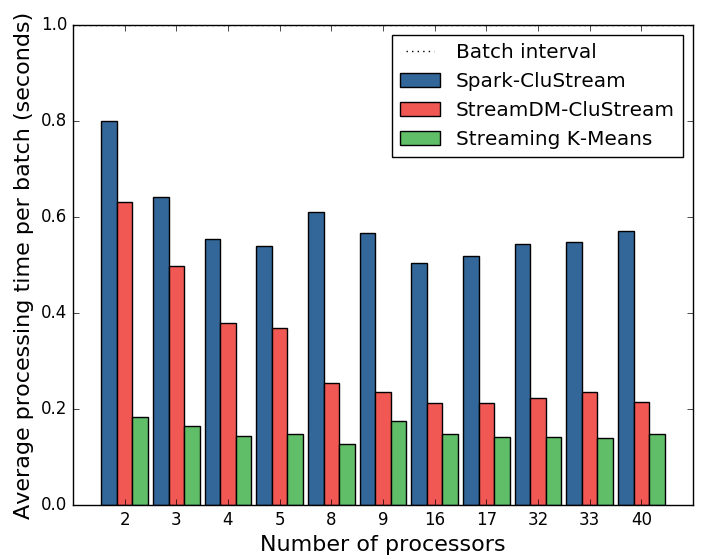
\includegraphics[scale=0.45]{./styles/perfComp2.png}
 \caption{Processing time comparison: $q=20$, $d=2$}
 \label{fig:perfComp2}
\end{figure}

In Figure \ref{fig:perfComp2} it can be seen that \textit{Spark-CluStream} took the most time on average to process a batch of data and being \textit{Streaming K-Means} the fastets among the three. 

\begin{figure}[h!]
 \centering
 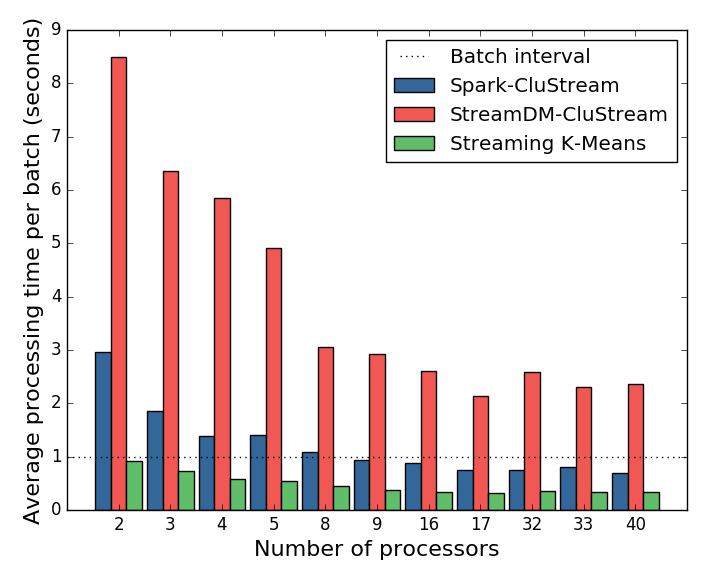
\includegraphics[scale=0.45]{./styles/perfComp100.png}
 \caption{Processing time comparison: $q=20$, $d=100$}
 \label{fig:perfComp100}
\end{figure}

When it comes to higher dimensions, \textit{Spark-CluStream} shows a significant improvement over \textit{StreamDM-CluStream}, which never got to the point were it was stable (below the 1 second mark), as shown in \ref{fig:perfComp100}, it seems to scale as fast as \textit{Spark-CluStream} but it was not enough even with 40 processors. 


\begin{figure}[h!]
 \centering
 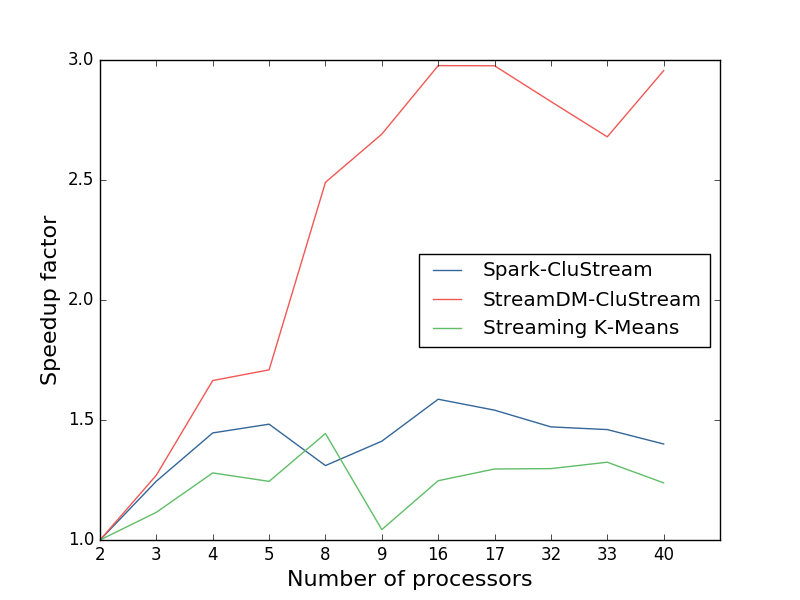
\includegraphics[scale=0.45]{./styles/scalComp2.png}
 \caption{Scalability comparison: $q=20$, $d=2$}
 \label{fig:scalComp2}
\end{figure}

Surprisingly, in Figure \ref{fig:scalComp2}, \textit{StreamDM-CluStream} shows to be able to scale even for this tests, while both \textit{Spark-CluStream} and \textit{Streaming K-Means} seem to struggle taking advantage of using more processors.

\begin{figure}[h!]
 \centering
 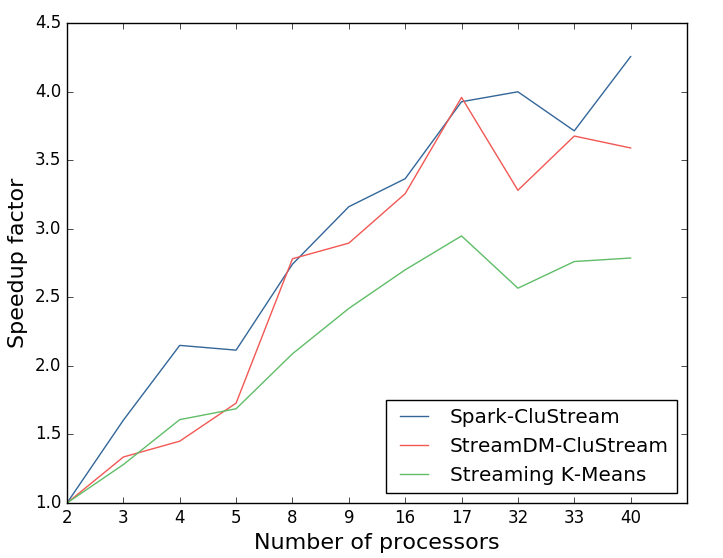
\includegraphics[scale=0.45]{./styles/scalComp100.png}
 \caption{Processing time comparison: $q=20$, $d=100$}
 \label{fig:scalComp100}
\end{figure}

Figure \ref{fig:scalComp100} shows that all three algorithms are able to scale similarly for this test, being \textit{Spark-CluStream} the one having a very slight advantage as it does not slow down as quickly as the other two.



Another interesting comparison, is the processing time per batch of data for a single machine, using a real dataset such as the \textit{Network Intrusion}. Here, communication is less of an issue as all the partitions lie in the same share memory space, and still there are 4 virtual cores in disposition for the algorithms to run. 

The test was performed using a stream speed of 2000 points per batch and with a horizon $H=1$, to match one of the validation tests.

\begin{figure}[h!]
 \centering
 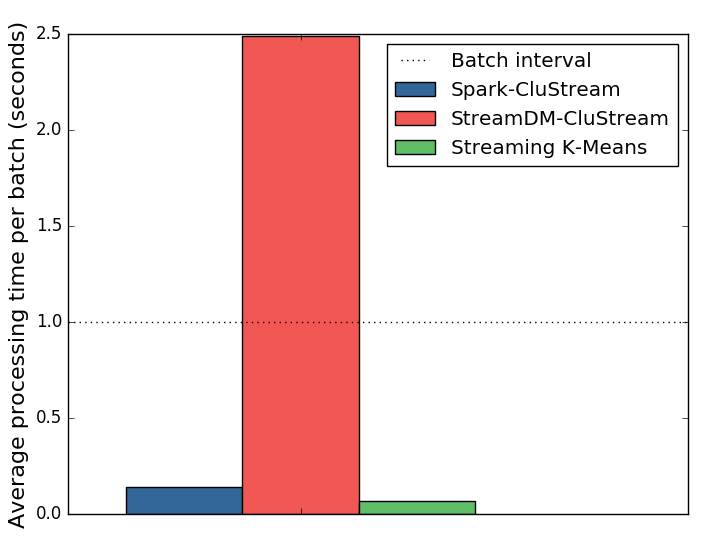
\includegraphics[scale=0.47]{./styles/singlemachine.png}
 \caption{Processing time comparison for a single machine: $q=50$, $d=34$}
 \label{fig:singlemachine}
\end{figure}

The results shown in Figure \ref{fig:singlemachine} are quite remarkable. As \textit{StreamDM-CluStream} shows a very significant disadvantage when using greater numbers of micro-clusters and higher dimensions.

For this single machine test, \textit{Spark-CluStream} was about 18 times faster on average than \textit{StreamDM-CluStream} and about two times slower than \textit{Streaming K-Means} on average.

Another consideration to be made, is that  \textit{Spark-CluStream} saves a snapshot for every batch of data, having to write to disk, while the other two algorithms never access the disk or this matter.


